\section{Теория графов}

Графы — это фундаментальное понятие в дискретной математике, и теория графов играет важную роль в изучении различных аспектов их применения. Графы используются для моделирования и анализа множества реальных явлений, таких как сети, маршрутизация, социальные взаимодействия и многое другое.

В этом разделе мы рассмотрим основные понятия теории графов, которые помогут нам заложить базис для дальнейшего изучения этой темы.

\subsection{Основные определения}

Графы обеспечивают эффективное средство для описания бинарных отношений между различными объектами. Чтобы понять эту концепцию, можно взять пример из социальной сети: люди в этой сети представляют собой множество объектов, обозначаемых как $V$. В то же время отношения между этими людьми, такие как подписки или дружба, можно рассматривать как набор бинарных связей. Если объект $v_i$ подписан на объект $v_j$, это означает наличие определенной связи между этими двумя людьми.

Для визуализации графов часто используется графическое представление, в котором объекты изображаются в виде кругов или узлов, а связи между ними – в виде линий или рёбер. Такой способ визуализации помогает лучше понять структуру графа и позволяет легче выявлять взаимосвязи между различными элементами.

В теории графов мы можем классифицировать графы по их структуре и направленности. Граф считается ориентированным, если он содержит непустое множество вершин $V$ и множество отношений или рёбер $E \subset V \times V$, при этом каждое ребро можно трактовать как упорядоченную пару $(v_i, v_j)$. Это означает, что в ориентированном графе направление связи между вершинами имеет значение. В данном случае, если в графе есть ребро из вершины $v_i$ в вершину $v_j$, то может не быть обратного ребра из $v_j$ в $v_i$. Такой граф часто называют "ориентированным графом" или "диграфом".

Если же граф содержит симметричные отношения между вершинами, он называется неориентированным. В неориентированном графе наличие ребра между вершинами $v_i$ и $v_j$ означает, что связь двусторонняя: если есть ребро $(v_i, v_j)$, то автоматически имеется и обратное ребро $(v_j, v_i)$.

Существует также класс графов, называемых смешанными графами. Они обладают одновременно ориентированными и неориентированными рёбрами, что придаёт им более сложную структуру и позволяет описывать более разнообразные ситуации.

На рисунке \ref{fig:digraph} представлен пример различных типов графов, показывающий, как можно визуально различать ориентированные, неориентированные и смешанные графы. Такой подход к изображению графов позволяет легко понять, какой тип отношений присутствует в каждом конкретном случае.

\begin{figure}[H]
	\begin{center}
		 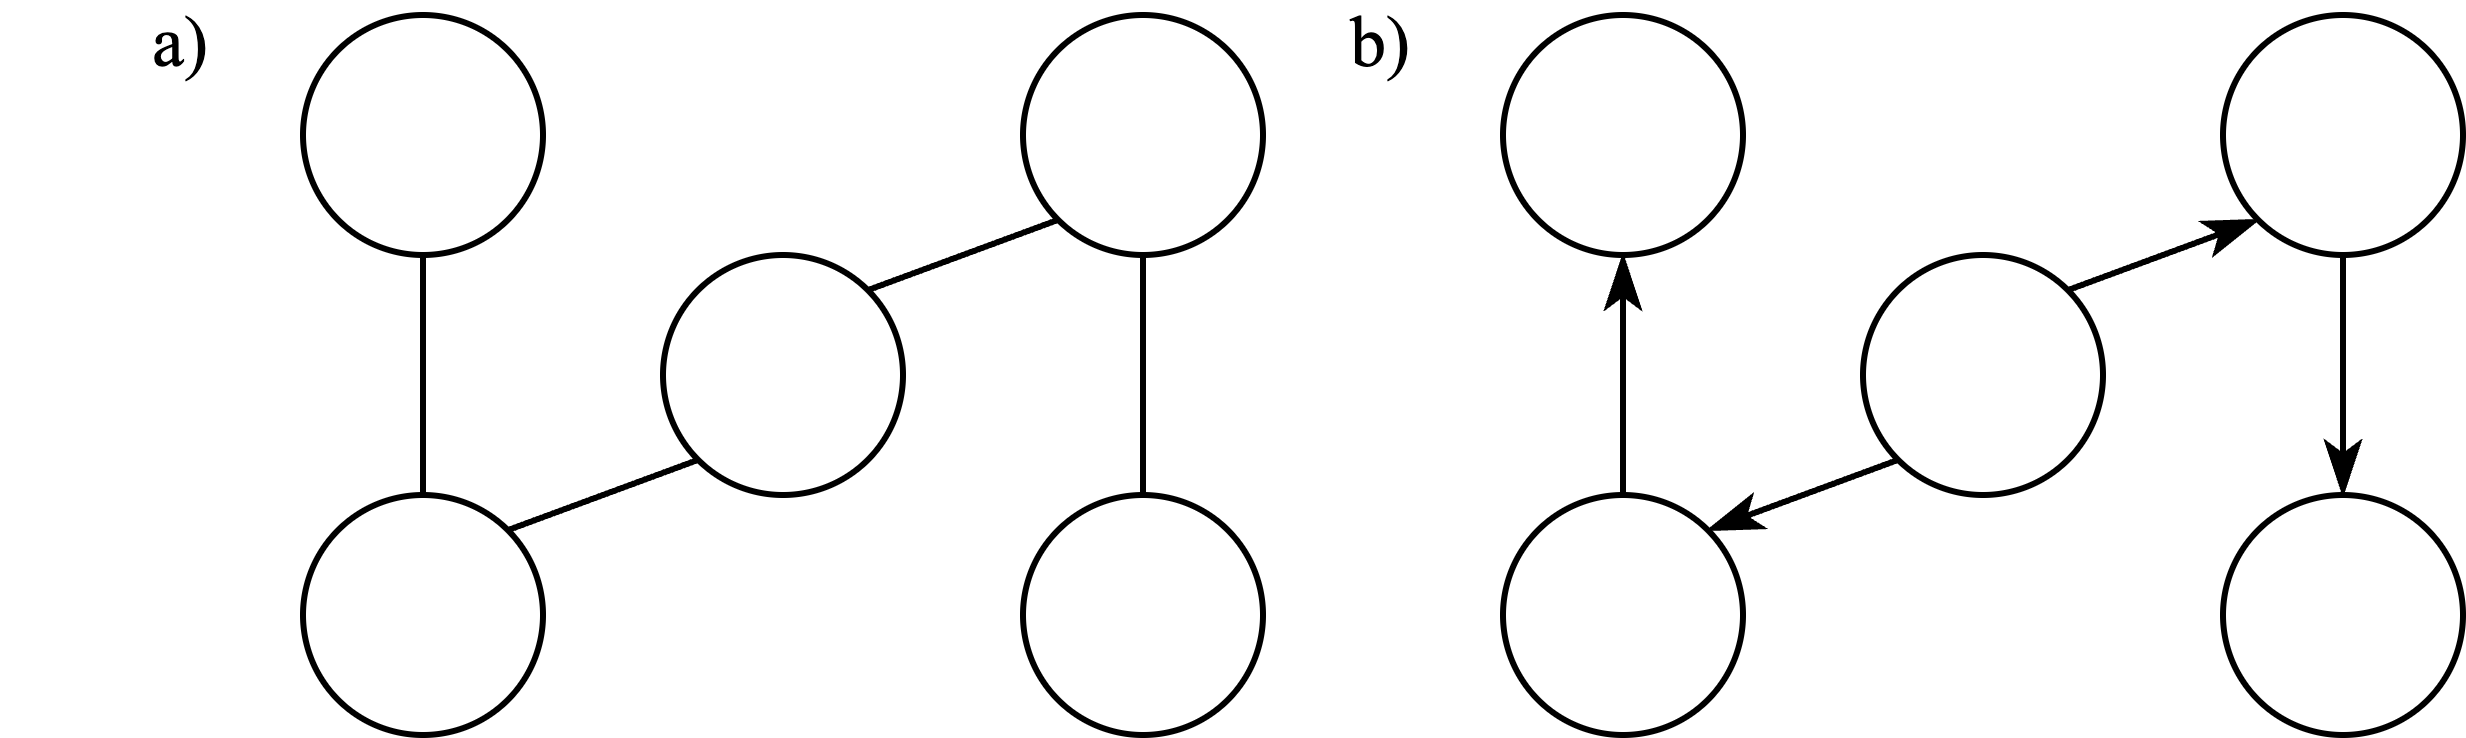
\includegraphics[width=0.7\linewidth]{src/img/1/digraph.png}
		 \caption{Ориентированный граф (a), неориентированный граф (b)}
		\label{fig:digraph}
	\end{center}
\end{figure}

Полный граф — это граф, в котором каждая вершина соединена со всеми другими вершинами. Это означает, что множество рёбер $E$ эквивалентно декартовому произведению множества вершин $V \times V$. В таком графе между любой парой вершин существует прямое отношение или ребро, что создает сеть с максимальной плотностью связей. Полные графы часто используются в различных теоретических моделях и имеют ряд интересных свойств.

Взвешенный граф — это граф, в котором каждому ребру или вершине присваивается некоторый вес или значение. Этот вес может представлять что угодно: от стоимости или длины пути до количества ресурсов или времени, необходимого для преодоления данного ребра или для работы с данной вершиной. Взвешенные графы позволяют анализировать графы с учетом дополнительных параметров и часто используются для задач, связанных с оптимизацией.

Путь в графе — это последовательность рёбер, которая соединяет ряд вершин, начиная с исходной вершины и заканчивая конечной. Формально, путь определяется как набор рёбер $E_1, E_2, \ldots, E_n$, где конечная вершина одного ребра совпадает с начальной вершиной следующего. Путь считается простым, если никакое ребро не повторяется более одного раза. Элементарный путь — это путь, в котором каждая вершина посещается только один раз, что означает отсутствие повторяющихся вершин.

Цикл — это особый тип пути, который начинается и заканчивается в одной и той же вершине. Если граф является направленным, цикл может называться контуром. Циклы важны для выявления повторяющихся процессов или замкнутых систем в графе.

На изображении \ref{fig:path_example} показан пример пути, который является простым, поскольку каждое ребро используется только один раз, но не элементарным, так как центральная вершина посещается дважды. Такие примеры иллюстрируют различия между простыми и элементарными путями и показывают, как они могут применяться в различных контекстах анализа графов.


\begin{figure}[H]
	\begin{center}
		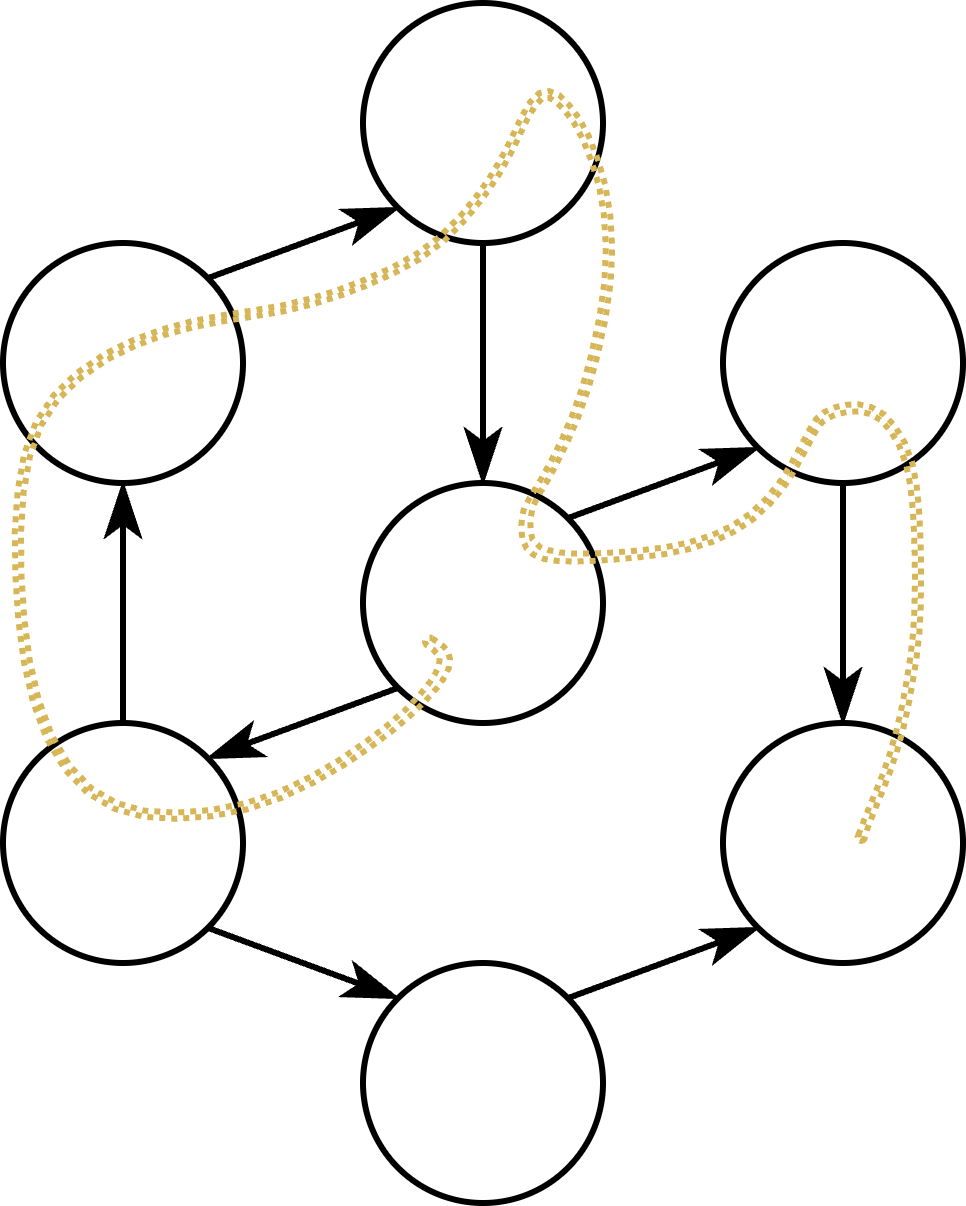
\includegraphics[width=0.3\linewidth]{src/img/1/graph_path.png}
		\caption{Простой, но не элементарный путь в графе}
		\label{fig:path_example}
	\end{center}
\end{figure}

Граф считается связным, если для каждой пары различных вершин в этом графе существует хотя бы один путь, соединяющий их. Это означает, что в связном графе можно переместиться из любой вершины к любой другой, следуя по рёбрам, которые соединяют вершины.

Связность является ключевым свойством графов, которое определяет их структуру и характер. В связном графе все вершины так или иначе соединены друг с другом, даже если путь между ними может проходить через другие промежуточные вершины.

Связные графы часто используются для моделирования систем, в которых элементы имеют некоторую степень взаимодействия или зависимости. Например, в социальной сети связный граф указывает на то, что существует путь коммуникации между любыми двумя участниками сети, даже если они могут быть связаны через нескольких посредников.

Если граф не является связным, то он состоит из нескольких отдельных компонент, каждая из которых представляет собой связный граф. Эти компоненты могут быть изучены отдельно, так как они не имеют связей друг с другом. Исследование связности графов позволяет выявлять изолированные сегменты или группы тесно связанных элементов.


\subsection{Изоморфизм графов}


Изоморфизм в теории графов — это понятие, которое указывает на структурное сходство между графами. Когда говорят, что графы $G_1$ и $G_2$ изоморфны, это означает, что между ними можно установить взаимно однозначное соответствие для вершин и рёбер. Иными словами, если имеется биекция между вершинами двух графов, которая сохраняет структуру рёбер, то такие графы считаются изоморфными.

Изоморфизм графов подразумевает, что их визуальная структура может отличаться, но по сути они идентичны. Например, если у одного графа вершины $A, B, C$ соединены рёбрами в определенной последовательности, то в другом графе можно найти соответствие, в котором другие вершины $X, Y, Z$ имеют те же рёбра в той же последовательности. Изоморфизм позволяет понять, когда два графа, несмотря на различие в именах или представлениях, имеют одинаковую структуру.

Подграфы — это части графа, которые включают некоторую подмножество вершин и рёбер из исходного графа. Если два подграфа из разных графов изоморфны друг другу, то их называют изоморфными подграфами. Такое понятие полезно при анализе сложных графов, когда нужно найти общие структуры или повторяющиеся паттерны.

Двойной изоморфизм подграфов — это ситуация, в которой два разных графа содержат подграфы, которые изоморфны друг другу. Это более широкий концепт, который указывает на то, что в двух графах есть общие структуры, но сами графы при этом могут не быть изоморфными.

Таким образом, изоморфизм и его вариации позволяют исследовать и выявлять структурное сходство в графах, что часто используется в таких областях, как компьютерные науки, биоинформатика и теория сетей.


\subsection{Деревья}

Деревья представляют собой особый вид графов, которые широко применяются в различных областях информационных технологий, таких как алгоритмы, структуры данных. В этой работе деревья будут служить основой для алгоритмов генерации маршрутов.

Подобно графам, деревья делятся на два класса: ориентированные и неориентированные. Неориентированное дерево — это связный граф, который не содержит простых циклов. Это означает, что если начать обход по дереву из любой вершины, невозможно вернуться к исходной точке, не пройдя по рёбрам назад. Деревья уникальны своей структурой, поскольку они всегда связаны, но не имеют замкнутых путей.

В деревьях есть особые вершины, которые называются листовыми. Листовые вершины — это вершины, которые имеют степень, равную единице, то есть из них выходит только одно ребро. Они представляют собой конечные точки в дереве, и их наличие указывает на то, что это дерево имеет четко определенную структуру без циклов.

Остальные вершины в дереве, из которых выходит более одного ребра, называются внутренними вершинами. Внутренние вершины обеспечивают структуру дерева, соединяя между собой другие вершины и образуя пути, которые могут вести к листовым вершинам.

В целом, деревья обладают рядом полезных свойств, которые делают их ключевым элементом в алгоритмах, особенно тех, что связаны с обработкой данных, маршрутами и поиском путей. Их использование в алгоритмах генерации маршрутов позволяет оптимизировать процесс поиска и обеспечить целостность структуры данных.

В теории алгоритмов и структур данных распространены так называемые деревья поиска. Деревом поиска называется дерево, в каждой вершине которого находятся 2 объекта (ключ и значение). 






\subsection{Расстояния на графе}

\subsection{Раскраска графов}

\subsection{Эйлеровы и гамильтоновы графы}

\subsection{Кратчкайшие пути на графе}


\section{Теория вероятности}

\subsection{Основные определения}

\subsection{Случайные переменные}

\subsection{Теория информации}


\section{Интеллектуальный анализ с помощью теории графов}



\section{Вероятностные модели}

\subsection{Байесовсеие классификаторы}

\subsection{Скрытые марковские модели}

\subsection{Марковские случайные поля}

\subsection{Байесовские сети}


\section{Модели принятия решений}

\subsection{Графы принятия решений}


\section{Варианты хранения взаимосвязанных данных}


\section{Моделирование данных графами}


\section{Внутреннее устройство графовых баз данных}

%-------------
%
%- глава 1
%основы теории графов (основные определения)
%расстояния на графе (диаметр, центр, радиус)
%нагруженные графы, кратчайшее расстояние на графе
%раскарска графов
%эйлеровы и гамильтоновы графы
%
%- глава 2
%основные понятия теории вероятнос
%
%-------------
%
%Многие ситуации в реальном мире могут быть удобно описаны с помощью диаграммы, состоящей из набора точек и линий, соединяющих определенные пары этих точек. Например, точки могут представлять людей, а линии могут отображать соединяющие пары друзей; или точки могут быть центрами связи, а линии - каналами связи. Обратите внимание, что на таких диаграммах в основном интересует, соединены ли две заданные точки линией или нет; способ, которым они соединены, не имеет значения. Математическая абстракция ситуаций такого типа приводит к появлению концепции графа. Граф $G$ - это упорядоченная тройка $(V (G), E (G),4G)$, состоящая из непустого множества вершин $V(G)$, множества ребер $E(G)$, не пересекающихся с $V(G)$, и функции инцидентности, которая связана с каждым ребром графа $G$ неупорядоченная пара (не обязательно различных) вершин $G$. Если $e$ - ребро, а $u$ и $v$ - вершины, такие, что $G(e) = uv$, то говорят, что $e$ соединяет $u$ и $v$; вершины $u$ и $v$ называются концами $e$. Для пояснения определения следует привести два примера графов.
%
%Теория графов представляет собой обширную область математики, которая изучает структуры, состоящие из вершин и рёбер, а также их свойства. В контексте разработки рекомендательной системы для генерации маршрутов, где необходимо учитывать фиксированную дистанцию, а также пользовательские фильтры, понимание основных концепций теории графов имеет важное значение. Данный раздел представляет обзор ключевых аспектов теории графов и их применение.
%
%Истоки теории графов уходят в XVIII век, когда математики начали исследовать проблемы, связанные с сетями, коммуникациями и транспортными системами. Одним из первых, кто активно развивал теорию графов, был Леонард Эйлер. В 1736 году он опубликовал статью, в которой предложил общий метод решения задач о прохождении мостов, представив карту Кёнигсберга в виде графа. Это и стало началом развития теории графов как самостоятельной математической дисциплины.
%
%%В дальнейшем теория графов развивалась благодаря работам таких учёных, как Аугустин Кайршль, Петер Гюйгенс, Уильям Роуан Хэмилтон и других. Важным вехом стала работа Артура Кэли и Фрэнсиса Киркмана, которые в 1857 году опубликовали теорему о связности графов.
%%
%%В XX веке теория графов получила новый импульс развития благодаря работам таких учёных, как Клод Берж, Джордж Полиа, Дейвид Кёниг, Пол Эрдёш, Джон Хопкрофт и Роберт Тарьян, которые внесли значительный вклад в область алгоритмов, комбинаторики и приложений теории графов.
%
%С появлением компьютеров и развитием информационных технологий теория графов стала не только важным математическим инструментом, но и активно применяется в практических областях, таких как компьютерные сети, социальные сети, биоинформатика, логистика и другие. Её методы и подходы стали неотъемлемой частью современной науки и техники.
%
%%\subsection{Задача о кёнигсбергских мостах}
%
%d
%
%%\subsection{Задача о четырёх красках}
%
%d
%
%%\subsection{Основные объекты теории графов}
%
%Дадим определение основным объектам теории графов.
%
%\begin{itemize}
%	\item графом G называется пара $(V,E)$, где $V$ - множество вершин (узлов), а $E$ - множество рёбер (связей) между этими вершинами.
%	\item Ориентированный и неориентированный графы: В неориентированном графе рёбра не имеют направления, в то время как в ориентированном каждое ребро имеет направление от одной вершины к другой.
%	\item Путь - последовательность вершин, в которой каждая пара соседних вершин соединена ребром.
%	\item Цикл - путь, в котором начальная и конечная вершины совпадают.
%	\item Граф называется связным, если между любыми двумя его вершинами существует путь.
%	\item Для неориентированных графов степень вершины - это количество рёбер, связанных с данной вершиной. В ориентированных графах учитываются входящие и исходящие рёбра.
%	\item Подграф графа $G$ - это граф, вершины и рёбра которого являются подмножествами вершин и рёбер графа $G$.
%	\item Деревья: Дерево - это связный граф без циклов. Каждая вершина в дереве имеет ровно одну входящую связь, за исключением корневой вершины, которая не имеет входящих связей.
%	\item Матрица смежности и список смежности: Матрица смежности - это квадратная матрица, где элемент $a_{ij}$ равен $1$, если между вершинами $i$ и $j$ есть ребро, и $0$ в противном случае. Список смежности представляет граф в виде списка, где каждая вершина сопоставляется со списком вершин, с которыми она связана.
%\end{itemize}
%
%Эти основные концепции теории графов обеспечивают базовый фреймворк для анализа и решения различных задач, связанных с графами. В дальнейших главах данной работы будут исследованы более сложные алгоритмы и приложения, использующие графовые структуры.
%
%
%%\subsection{Основные теоремы и их следствия}
%
%\begin{itemize}
%	\item Теорема о связности графа:
%	
%	Результат: Граф является связным тогда и только тогда, когда между любыми двумя его вершинами существует путь.
%	
%	Применение: Определение связности играет ключевую роль в различных задачах, таких как сетевой маршрутизации, поиск компонент связности в графах и многих других.
%	
%	\item Теорема Эйлера о планарных графах:
%	
%	Результат: Планарный граф может быть нарисован на плоскости так, чтобы его рёбра не пересекались.
%	
%	Применение: Эта теорема полезна в проектировании схем схемотехники, дорожных сетей и других структур, где важно избегать пересечений.
%	
%	\item Теорема о минимальном остовном дереве (МОД):
%	
%	Результат: Для связного неориентированного графа с весами на рёбрах существует уникальный МОД, содержащий все вершины графа и имеющий минимальную сумму весов рёбер.
%	
%	Применение: Применяется в задачах оптимизации, таких как минимальное остовное дерево в сетях связи и транспортных сетях.
%	
%	\item Теорема о потоках и разрезах (теорема Форда-Фалкерсона):
%	
%	Результат: Для любого потока в графе максимальный поток равен минимальному разрезу.
%	
%	Применение: Используется для решения задач максимального потока и минимального разреза в сетях, таких как транспортные сети и сети электропередачи.
%	
%	\item Теорема о четности степеней вершин в неориентированных графах:
%	
%	Результат: В неориентированном графе количество вершин нечетной степени всегда четно.
%	
%	Применение: Эта теорема используется в различных задачах, включая проверку наличия эйлерова цикла в графе.
%	
%	\item Теорема о цветовой раскраске графа (теорема о четырёх красках):
%	
%	Результат: Любой плоский граф может быть правильно раскрашен с использованием не более четырёх различных цветов.
%	
%	Применение: Применяется в картографии для раскрашивания карт так, чтобы соседние регионы имели разные цвета, и в различных задачах графического моделирования, требующих минимизации числа используемых цветов.
%	
%	\item Теорема Кёнига о покрытиях в двудольных графах:
%	
%	Результат: В каждом двудольном графе количество рёбер в минимальном покрытии равно числу вершин в максимальном паросочетании.
%	
%	Применение: Используется в задачах оптимизации, например, в различных алгоритмах для планирования расписания, а также в теории сетей для оптимизации распределения ресурсов.
%	
%	\item Теорема Холла о паросочетаниях:
%	
%	Результат: Для любого двудольного графа G с долями X и Y существует паросочетание, покрывающее все вершины X, если и только если для любого подмножества вершин S из X мощность множества соседей $N(S)$ больше или равна мощности S.
%	
%	Применение: Используется в задачах, связанных с назначением ресурсов или соединений в сетях, таких как задачи назначения ресурсов и соединений в сетях транспортировки или коммуникаций.
%	
%	\item Теорема Меньгера:
%	
%	Результат: В неориентированном графе минимальное количество вершин, разделяющих две заданные вершины s и t, равно максимальному количеству непересекающихся путей между s и t.
%	
%	Применение: Используется в задачах нахождения наиболее эффективных маршрутов, например, в транспортной логистике или сетях связи.
%	
%	\item Теорема Дирака о гамильтоновых циклах:
%	
%	Результат: Если в графе G с n вершинами каждая вершина имеет степень не менее n/2, то граф содержит гамильтонов цикл.
%	
%	Применение: Применяется в задачах, требующих нахождения замкнутых маршрутов, таких как в области транспортировки или проектировании эффективных обходов для механизмов.
%	
%	\item Теорема Мостов Кёнига о деревьях:
%	
%	Результат: В любом связном графе с $n$ вершинами $n-1$ ребро является достаточным и необходимым условием для того, чтобы он был деревом.
%	
%	Применение: Эта теорема используется для проверки наличия циклов в графах и в задачах поиска минимальных остовных деревьев.
%	
%	\item Теорема Штайнера:
%	
%	Результат: Для заданных точек на плоскости (называемых узлами) и некоторого числа дополнительных точек (называемых точками Штайнера) существует граф, содержащий только данные точки и имеющий минимальную длину.
%	
%	Применение: Эта теорема используется в различных задачах, таких как проектирование схем коммуникаций или сетей, где нужно минимизировать длину кабелей или стоимость связи.
%	
%	\item Теорема Турана о толстых подграфах:
%	
%	Результат: Для любого графа с n вершинами и без треугольников максимальное количество рёбер ограничено сверху.
%	
%	Применение: Эта теорема используется в задачах, связанных с поиском плотных подграфов или определением верхней границы количества рёбер в графе.
%\end{itemize}
%
%%\subsection{Приложения теории графов}
%
%\begin{itemize}
%	\item Социальные сети: Социальные сети можно представить в виде графов, где узлы представляют пользователей, а рёбра - связи между ними. Анализ графа социальной сети позволяет исследовать структуру сети, выявлять влиятельных пользователей, группы схожих интересов и т. д.
%	
%	\item Маршрутизация в компьютерных сетях: Графы используются для моделирования компьютерных сетей, где узлы представляют маршрутизаторы или узлы сети, а рёбра - связи между ними. Различные алгоритмы маршрутизации, такие как алгоритм Дейкстры или алгоритм Беллмана-Форда, используются для нахождения оптимальных путей между узлами сети.
%	
%	\item Биоинформатика: Графы используются для моделирования биологических сетей, таких как генетические сети, белковые взаимодействия и др. Анализ таких графов позволяет исследовать сложные взаимодействия в биологических системах и выявлять ключевые элементы.
%	
%	\item Маршрутизация и логистика: В транспортной логистике графы используются для моделирования сетей дорог, железных дорог, авиалиний и т. д. Алгоритмы маршрутизации помогают оптимизировать распределение грузов и пассажирские перевозки, минимизируя время и затраты.
%	
%	\item Финансовая аналитика: Графы могут использоваться для моделирования финансовых сетей, таких как сети финансовых учреждений, банковских транзакций или связей между компаниями. Анализ таких сетей позволяет выявлять системные риски, связанные с финансовыми кризисами и колебаниями на рынке.
%	
%	\item Графовые базы данных: Графовые базы данных используются для хранения и анализа связанных данных, таких как социальные сети, транспортные сети, биологические сети и др. Они предоставляют эффективные методы для выполнения запросов и анализа связанных данных.
%	
%	\item Оптимизация процессов: Графы используются для моделирования процессов в производстве, логистике, телекоммуникациях и других отраслях. Анализ графа позволяет оптимизировать производственные процессы, управлять инвентаризацией, распределением ресурсов и др.
%	
%	\item Робототехника и навигация: Графы используются для моделирования окружающей среды роботов и планирования их движения. Алгоритмы поиска пути и управления роботами основаны на анализе графов для эффективного перемещения в пространстве.
%\end{itemize}
%
%
%%\subsection{Алгоритмы на графах}
%
%Рассмотрим несколько ключевых алгоритмов на графах, которые широко используются в различных областях:
%
%\begin{itemize}
%	\item Алгоритм поиска в ширину (BFS):
%	
%	Описание: BFS исследует граф от заданной стартовой вершины, поочередно обходя все ближайшие к ней вершины, затем переходя к следующему уровню.
%	Применение: Используется для поиска кратчайшего пути в невзвешенном графе, определения связности графа, поиска кратчайшего пути в графе, представленном в виде дерева, и др.
%	
%	\item Алгоритм поиска в глубину (DFS):
%	
%	Описание: DFS исследует граф до тех пор, пока не достигнет конечной вершины, а затем возвращаетсть назад и продолжает поиск.
%	Применение: Используется для нахождения компонент связности в графе, топологической сортировки, поиска циклов в графе, проверки наличия пути между вершинами и др.
%	
%	\item Алгоритм Дейкстры:
%	
%	Описание: Алгоритм Дейкстры находит кратчайший путь от одной вершины графа до всех остальных, при условии, что веса рёбер неотрицательны.
%	Применение: Используется для поиска кратчайших путей в графах с весами, например, в сетях передачи данных, транспортных сетях и т. д.
%	
%	\item Алгоритм Беллмана-Форда:
%	
%	Описание: Алгоритм Беллмана-Форда находит кратчайшие пути от одной вершины графа до всех остальных, даже при наличии рёбер с отрицательным весом, но не содержащих отрицательные циклы.
%	Применение: Используется для нахождения кратчайших путей в графах с весами, где могут присутствовать рёбра с отрицательным весом, но нет отрицательных циклов.
%	
%	\item Алгоритм Прима:
%	
%	Описание: Алгоритм Прима находит минимальное остовное дерево взвешенного связного графа.
%	Применение: Используется в задачах минимизации стоимости, таких как проектирование сетей передачи данных, планирование транспортных маршрутов и др.
%	
%	\item Алгоритм Крускала:
%	
%	Описание: Алгоритм Крускала также находит минимальное остовное дерево, но он работает не построением дерева, а пошаговым добавлением рёбер с минимальным весом, не образующих цикл.
%\end{itemize}
%
%Применение: Используется в задачах оптимизации, связанных с построением минимальных сетей связи, электропередачи и др.
%Эти алгоритмы являются лишь некоторыми из множества методов и подходов, применяемых в теории графов для решения различных задач. Каждый из них имеет свои особенности и применяется в зависимости от требований и характеристик конкретной задачи.
%
%
%%\section{Вероятностные графовые модели}
%
%d
%
%%2.1 Пути и циклы в графах
%%Пути и циклы - это основные элементы, используемые для описания путей перемещения в графах.
%
%%Пути: Путь в графе представляет собой последовательность вершин, в которой каждая вершина соединена ребром с последующей вершиной. Путь может быть простым или составным, в зависимости от наличия повторяющихся вершин.
%%Циклы: Цикл в графе - это путь, в котором начальная и конечная вершины совпадают, и ни одна вершина не повторяется, кроме начальной и конечной. Они могут быть простыми или составными, а также могут иметь различные свойства, влияющие на структуру графа и возможные маршруты.
%%2.2 Изоморфизм и деревья в графах
%%Изоморфизм и деревья - это концепции, которые помогают понять структуру и связи между вершинами в графах.
%
%%Изоморфизм графов: Графы называются изоморфными, если существует биективное отображение между их множествами вершин, сохраняющее отношение смежности. Понимание изоморфизма позволяет выявлять схожие или одинаковые паттерны в различных сетевых структурах.
%%Деревья: Дерево - это связный ациклический граф. Они играют важную роль в моделировании иерархических структур и имеют широкое применение в алгоритмах маршрутизации и анализе данных.
%%2.3 Клики и полное упорядочивание графов
%%Клики и полное упорядочивание графов представляют собой дополнительные аспекты структуры графов.
%
%%Клики: Клика - это подграф, в котором каждая вершина соединена с каждой другой вершиной. Клики играют важную роль в анализе социальных сетей и обнаружении сообществ.
%%Полное упорядочивание: Полное упорядочивание - это такое отношение порядка на множестве вершин, при котором для любых двух вершин одна из них достижима из другой. Понимание полного упорядочивания важно для анализа структуры графа и применимости различных алгоритмов.
%%2.4 Алгоритмы упорядочивания и триангуляции графов
%%Алгоритмы упорядочивания и триангуляции позволяют анализировать и оптимизировать графы для эффективной работы рекомендательных систем.
%
%%Алгоритмы упорядочивания: Существует множество алгоритмов для упорядочивания графов, таких как алгоритм Тарьяна и алгоритм Хопкрофта-Тарьяна, которые находят применение в различных областях, включая географическую информационную систему (ГИС) и компьютерную графику.
%%Триангуляция графов: Триангуляция позволяет разбить граф на треугольники, что упрощает анализ и обработку данных. Она широко используется в графических системах и вычислительной геометрии.